\section{Experimental Studies}
\label{sec:experiments}

% NOTE: This section is written for the main paper. It emphasizes the empirical
% claims and defers implementation details to the appendix file
% paper/experiments_appendix.tex.

\paragraph{Setup.}
We evaluate the theory in a controlled frozen-teacher linear-Gaussian setting.
Each example is generated from a latent state $s\sim\mathcal{N}(0,I_{r_\star})$,
a context view $z=Cs+\sigma_z\epsilon_z$, and $K$ target embeddings
$y_k=A_ks+\sigma_y\epsilon_k$. The context operator
$C\in\mathbb{R}^{D_x\times r_\star}$ is a fixed random orthonormal frame
($C^\top C=I$), so the experiments isolate the role of target structure rather
than context-encoder conditioning. The stacked response is
$Y=(y_1^\top,\ldots,y_K^\top)^\top$, and the relevant population operator is the
stacked target-context covariance $\Sigma_{YZ}=AC^\top$ for the rank-growth
diagnostics. For the bottleneck and post-saturation diagnostics, the
theory-facing operator is the whitened raw predictor
$T_K=\Sigma_{YZ}^{(K)}\Sigma_{ZZ}^{-1/2}$.

\paragraph{Models.}
We compare the unconstrained ordinary least-squares predictor with its
rank-$d$ reduced-rank regression (RRR) truncation. The RRR rank $d$ plays the
role of the BM-JEPA embedding bottleneck. Because the teacher and context maps
are frozen and linear, this setting directly tests the rank, conditioning, and
spectral-tail mechanisms in the theory without confounding optimization or
encoder dynamics.

\paragraph{Data.}
The synthetic target bank separates two mechanisms. Target heterogeneity changes
the angular spread of a latent target dictionary, while target overlap changes
how concentrated the target-bank coverage is over that dictionary. Unless
otherwise stated, $r_\star=16$, $D_x=32$, and each target block is scalar. We use
ten deterministic seeds and report means with standard-error bands. The suite
summary in \cref{tab:experiment-summary} covers the four ablations, the
post-saturation diagnostic, and the fixed-trace predictive-isotropy ablation.
Additional generator and configuration details are reported in
\cref{app:experimental-details}.

\begin{table}[t]
\centering
\small
\begin{tabular}{lcccc}
\hline
Experiment & Sweep & Fixed quantities & Main outcome & Figure \\
\hline
$K$-saturation & $K$ & $d=r_\star$ & target-count saturation & \cref{fig:k-saturation} \\
Heterogeneity & $\widehat{\lambda}_{\mathrm{het}}$ & $K=32,\ d=16$ & finite-sample recovery & \cref{fig:heterogeneity} \\
Overlap & overlap $\omega$ & $K=24,\ d=16$ & redundancy failure mode & \cref{fig:overlap} \\
Bottleneck & $d$ & rich target bank & spectral-tail floor & \cref{fig:bottleneck} \\
Post-saturation & $K$ & $r_\star(K)=d$ & relative conditioning & \cref{fig:post-saturation} \\
Predictive isotropy & spectrum of $H_K$ & rank, trace, $K$ & fixed-trace isotropy & \cref{fig:predictive-isotropy} \\
Embed./pred. isotropy & spectra & rank, trace, $K$ & isotropy distinction & \cref{fig:embedding-vs-predictive-isotropy} \\
\hline
\end{tabular}
\caption{Synthetic experiment suite. All experiments use the same frozen
linear-Gaussian teacher family; only the indicated sweep variable changes.}
\label{tab:experiment-summary}
\end{table}

\paragraph{Metrics.}
All paper-facing risk panels use the average per-target normalization of
$\mathcal R_K$ in \eqref{eq:per_target_risk}. This is especially important for
the $K$-saturation and post-saturation sweeps, where the stacked target
dimension changes with $K$. In the heterogeneity experiment, we additionally
include a fixed-bank MSE probe on a common rich reference target bank. This
probe is not the canonical $\mathcal R_K$ risk; it asks whether the recovered
subspace transfers to a held-out complete target bank. Across the first three
ablations we also report recovered effective rank and the
heterogeneity/conditioning quantity
$\lambda_{\mathrm{het}}=\lambda_{\mathrm{rank}(G)}(G)$, where
$G=\Sigma_{ZY}\Sigma_{YZ}$ and has the same nonzero spectrum as the latent
target Gram matrix induced by $A$. In the heterogeneity experiment, the
horizontal axis is the measured finite-sample value
$\widehat{\lambda}_{\mathrm{het}}$, rather than the generator knob, so the plot
directly tests the paper's conditioning variable. Effective rank is computed by
counting singular values above $0.05$ of the largest singular value. Solid
curves show finite-sample estimates averaged over seeds; dashed curves show the
corresponding population values computed from the known synthetic operators.
For the bottleneck ablation, we additionally report the model effective rank,
the excess risk over OLS, and the normalized spectral-tail ratio
$\sum_{j>d}\sigma_j^2/\sum_j\sigma_j^2$ of the whitened population predictor.
For the predictive-isotropy ablation, we fix both rank and total predictive
energy and vary only the spectrum of
$H_K=T_K^\top T_K$. We report the relative conditioning
$\kappa_K^2=\lambda_d(H_K)/\lambda_1(H_K)$ and the normalized log-determinant
score
\[
    \frac{1}{d}\sum_{i=1}^d \log \lambda_i(H_K)
    -
    \log\left(\frac{1}{d}\sum_{i=1}^d \lambda_i(H_K)\right),
\]
which equals zero for a flat spectrum and becomes more negative as predictive
energy becomes anisotropic.

\paragraph{Baselines.}
The main baseline is the population counterpart of each finite-sample metric:
it is computed directly from the known operators $A$ and $C$, without sampling
noise. For the bottleneck experiment, unconstrained OLS is the reference model,
and the bottleneck spectral-tail result predicts that the excess risk of the rank-$d$ predictor is
governed by the spectral tail beyond the top $d$ predictive directions.

\paragraph{Results.}
The results in \cref{fig:k-saturation} support the target-count saturation claim:
per-target MSE decreases and recovered rank increases as complementary targets
are added, then both saturate once the available predictive rank is exhausted.
The results in \cref{fig:heterogeneity} show that larger measured
$\widehat{\lambda}_{\mathrm{het}}$ improves finite-sample recovery. The
canonical per-target risk $\mathcal R_K$ remains nearly flat because increasing
heterogeneity makes the target bank less redundant and therefore changes the
task being averaged. By contrast, fixed-bank MSE decreases because the learned
subspace transfers better to a common rich target bank; recovered rank rises and
the latent predictive structure becomes identifiable. The results in
\cref{fig:overlap} give the complementary failure mode: when target coverage
becomes redundant, increasing target overlap reduces effective rank and worsens
per-target MSE. Finally, \cref{fig:bottleneck} is consistent with the
bottleneck prediction: per-target MSE decreases with $d$, the learned model rank grows
as $\min\{d,r_\star\}$, and the finite-sample excess-risk ratio tracks both the
plug-in spectral-tail ratio and the population spectral-tail ratio. Together,
these results are consistent with the paper's
central message: multi-target prediction helps when targets expose
complementary predictive structure, but target redundancy and embedding
bottlenecks limit the attainable representation.
The diagnostic in \cref{fig:post-saturation} further separates rank growth from
post-saturation conditioning. Here the target bank is already full rank from
$K^\star=d$ onward, so additional targets cannot increase $r_\star(K)$. Instead,
targets allocated to weak predictive directions improve
$\kappa_K^2=\lambda_d(H_K)/\lambda_1(H_K)$ for
$H_K=T_K^\top T_K$ and reduce finite-sample error over a finite window, while
effective dimension, half-gap, and per-target risk-stability diagnostics remain
controlled. Panel (d) directly compares the per-target excess-risk left-hand
side with the empirical $\widehat L\|\sin\Theta_T\|_{\mathrm{op}}$ upper curve
from the subspace-Lipschitz excess-risk condition,
thereby exposing the recovery term used by the post-saturation corollary. The
calibrated concentration constant in \eqref{eq:post_saturation_epsilon} is
$\widehat C_{0.9}=1.49$ for $\delta=0.1$; panels (e) and (f) use this constant
with $\widehat L$ to plot the calibrated excess-risk and risk-decomposition
bounds from
\cref{cor:post_saturation_excess_risk_bound,cor:risk_decomposition}. The
half-gap condition in
\eqref{eq:post_saturation_half_gap} is empirically non-vacuous: with
$\widehat{\eta}_K
=\|\widehat T_K-T_K\|_{\mathrm{op}}/
\|T_K\|_{\mathrm{op}}$, the condition
$\widehat{\eta}_K\le \kappa_K/2$ holds for all deterministic runs in the
plotted sweep. At the weakest endpoint, $K=12$, we observe
$\widehat{\eta}_{\mathrm{mean}}=0.0469$,
$\widehat{\eta}_{\max}=0.0543$, and $\kappa_K/2=0.0707$. Appendix
\cref{app:experimental-details} gives the exact target-bank construction and
additional half-gap numerics.

Finally, \cref{fig:predictive-isotropy} tests the operator-level Gaussianity
prediction in the new predictive-isotropy section. In this experiment,
$r_\star=d$, $K=d$, and $\operatorname{tr}(H_K)$ are fixed across all
conditions; only the eigenvalue profile of $H_K$ changes. This isolates
predictive spectral allocation from rank growth and total signal strength. A
flat spectrum maximizes the entropy score and $\kappa_K^2$, while geometric
spectral decay makes the predictive signal increasingly anisotropic on its
rank-$d$ range. The observed $\|\sin\Theta_T\|_{\mathrm{op}}$ and common-bank
excess MSE both increase as the spectrum becomes less isotropic, consistent
with the finite-sample recovery mechanism. The training-bank per-target MSE is
nearly flat because the experiment holds total target energy fixed; this is the
intended control, not a failure mode. It shows that the recovery change is
driven by spectral balance rather than by more rank or more predictive energy.
Appendix \cref{fig:embedding-vs-predictive-isotropy} further separates
embedding-level isotropy from predictive isotropy by varying an embedding
covariance spectrum independently from the predictive spectrum. In that
diagnostic, common-bank excess risk is essentially unchanged by the embedding
isotropy score once the predictive spectrum is fixed, but changes by orders of
magnitude with $\kappa_K^2(T_K)$. This supports the interpretation that
embedding isotropy is at best a proxy, while the theory-facing quantity is the
operator-level isotropy of $H_K$.

% TODO: Verify the external theory label for the predictive-isotropy section.
% Suggested source label: sec:predictive-isotropy. The text above intentionally
% avoids relying on a guessed label until the theory source is synchronized.

% TODO: Verify theory labels before final paste:
% cor:post_saturation_relative_rate should point to Corollary 3.3.1.
% cor:post_saturation_excess_risk_bound should point to Corollary 3.3.2.
% cor:risk_decomposition should point to Corollary 3.3.3.
% eq:post_saturation_half_gap should point to the half-gap condition below the
% finite-window rate. If the rate equation itself has a label, reference it here
% as well rather than using literal equation numbers.

% INTERPRETATION: The experiments support the theory; they do not replace the
% formal statements. Keep causal language conservative in the final paper.

\begin{figure}[t]
    \centering
    
\includegraphics[width=\linewidth]{figures/exp_k_saturation.pdf}
    \caption{$K$-saturation under a fixed embedding bottleneck. Increasing the
    number of complementary target blocks lowers average per-target MSE and reveals
    additional predictive directions until the available predictive rank
    saturates.}
    \label{fig:k-saturation}
\end{figure}

\begin{figure}[t]
    \centering
    
\includegraphics[width=\linewidth]{figures/exp_heterogeneity.pdf}
    \caption{Effect of target heterogeneity. Larger measured
    $\widehat{\lambda}_{\mathrm{het}}$ reveals additional effective predictive
    rank. The per-target risk panel reports
    $\mathcal R_K$ on the changing target bank, while the fixed-bank panel
    probes transfer to a common rich target bank.}
    \label{fig:heterogeneity}
\end{figure}

\begin{figure}[t]
    \centering
    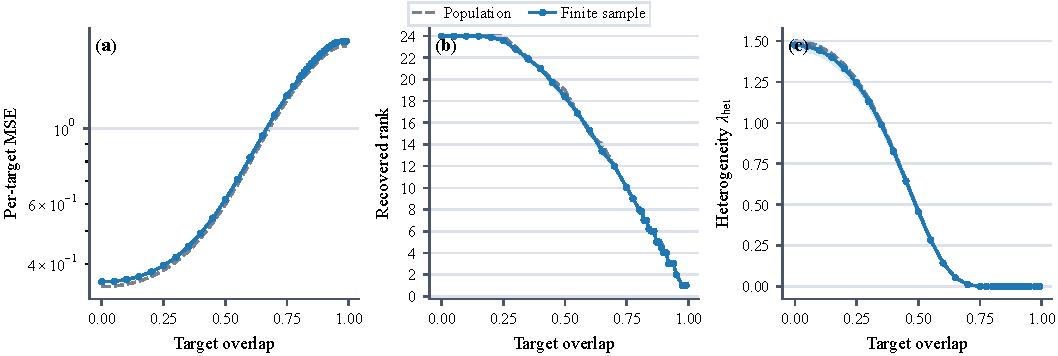
\includegraphics[width=\linewidth]{figures/exp_overlap.pdf}
    \caption{Effect of target overlap. Redundant targets reduce the
    heterogeneity/effective-rank gain expected from larger multi-target
    prediction objectives and worsen average per-target MSE.}
    \label{fig:overlap}
\end{figure}

\begin{figure}[t]
    \centering
    
\includegraphics[width=\linewidth]{figures/exp_bottleneck.pdf}
    \caption{Embedding bottleneck ablation. The target bank has latent
    predictive rank $r_\star=16$ while the allowed bottleneck rank $d$ is swept.
    Per-target MSE decreases as $d$ exposes more predictive directions. The model rank
    panel is expected to follow $\min\{d,r_\star\}$, while the normalized excess
    risk tracks the spectral-tail ratio and vanishes once $d\ge r_\star$.}
    \label{fig:bottleneck}
\end{figure}

\begin{figure}[t]
    \centering
    
\includegraphics[width=\linewidth]{figures/exp_post_saturation.pdf}
    \caption{Post-saturation relative-conditioning validation. The target bank
    is full rank from $K^\star=d$ onward, so $r_\star(K)=d$ throughout.
    Additional targets are allocated to weak predictive directions, increasing
    $\kappa_K^2=\lambda_d(H_K)/\lambda_1(H_K)$ for
    $H_K=T_K^\top T_K$ over a finite window. The first row reports
    eigenvalues of $H_K$, relative conditioning, and effective dimension of
    $T_K$; the second row reports the risk-stability bound, excess risk, and
    finite-sample risk. In panel (d), the solid curve is the empirical excess
    risk $\widehat{\mathcal R}_K-\mathcal R_K^\star$, while the dashed curve is
    $\widehat L\|\sin\Theta_T(V_K,\widehat V_K)\|_{\mathrm{op}}$. Here
    $\widehat L$ is the maximum of
    $[\widehat{\mathcal R}_K-\mathcal R_K^\star]_+/
    \|\sin\Theta_T(V_K,\widehat V_K)\|_{\mathrm{op}}$ over all deterministic seeds
    and all plotted $K$. Panel (e) compares the per-target excess risk with the
    calibrated excess-risk bound in
    \cref{cor:post_saturation_excess_risk_bound}. Panel (f) compares the
    finite-sample per-target risk $\widehat{\mathcal R}_K$ with the calibrated
    risk-decomposition bound in
    \cref{cor:risk_decomposition}. The half-gap condition in
    \eqref{eq:post_saturation_half_gap} is non-vacuous and holds in all
    deterministic runs in the plotted sweep.}
    \label{fig:post-saturation}
\end{figure}

\begin{figure}[t]
    \centering
    
\includegraphics[width=\linewidth]{figures/exp_predictive_isotropy.pdf}
    \caption{Predictive isotropy at fixed rank and fixed trace. All conditions
    have $r_\star=d=16$, $K=16$, and the same
    $\operatorname{tr}(H_K)$ for $H_K=T_K^\top T_K$; only the eigenvalue profile
    changes. A flatter spectrum gives larger $\kappa_K^2$, a larger
    log-determinant entropy score, smaller
    $\|\sin\Theta_T\|_{\mathrm{op}}$, and lower excess MSE on a common flat
    evaluation bank. The training-bank per-target MSE remains nearly unchanged
    because the total predictive energy is fixed by construction.}
    \label{fig:predictive-isotropy}
\end{figure}

% NOTE: Phase-2 real-data JEPA validation remains planned rather than claimed.
% A future version should add nonlinear encoders, EMA target encoders, image
% masks, representation probes, effective-rank diagnostics, and collapse tests.
